\providecommand{\setflag}{\newif \ifwhole \wholefalse}
\setflag
\ifwhole\else

% Typography and geometry ----------------------------------------------------
\documentclass[letterpaper]{scrbook}
\usepackage[inner=3cm,top=2.5cm,outer=3.5cm]{geometry}

\renewcommand\familydefault{bch}
\usepackage[utf8]{inputenc}
\usepackage{microtype}
\usepackage[small]{caption}
\usepackage[small]{titlesec}
\raggedbottom

% Graphics -------------------------------------------------------------------
\usepackage[pdftex]{graphicx}
\graphicspath{{_include/}}
\DeclareGraphicsExtensions{.png,.pdf}

% Code formatting ------------------------------------------------------------
\usepackage{fancyvrb}
\usepackage{courier}
\usepackage{listings}
\usepackage{color}
\usepackage{alltt}


\definecolor{comment}{rgb}{0.60, 0.60, 0.53}
\definecolor{background}{rgb}{0.97, 0.97, 1.00}
\definecolor{string}{rgb}{0.863, 0.066, 0.266}
\definecolor{number}{rgb}{0.0, 0.6, 0.6}
\definecolor{variable}{rgb}{0.00, 0.52, 0.70}
\lstset{
  basicstyle=\ttfamily,
  keywordstyle=\bfseries, 
  identifierstyle=,  
  commentstyle=\color{comment} \emph,
  stringstyle=\color{string},
  showstringspaces=false,
  columns = fullflexible,
  backgroundcolor=\color{background},
  mathescape = true,
  escapeinside=&&,
  fancyvrb
}
\newcommand{\code}[1]{\lstinline!#1!}
\newcommand{\f}[1]{\lstinline!#1()!}



% Links ----------------------------------------------------------------------

\usepackage{hyperref}
\definecolor{slateblue}{rgb}{0.07,0.07,0.488}
\hypersetup{colorlinks=true,linkcolor=slateblue,anchorcolor=slateblue,citecolor=slateblue,filecolor=slateblue,urlcolor=slateblue,bookmarksnumbered=true,pdfview=FitB}
\usepackage{url}

% Tables ---------------------------------------------------------------------
\usepackage{longtable}
\usepackage{booktabs}

% Miscellaneous --------------------------------------------------------------
\usepackage{pdfsync}
\usepackage{appendix}

\usepackage[round,sort&compress,sectionbib]{natbib}
\bibliographystyle{plainnat}


\title{ggplot2}
\author{Hadley Wickham}

\begin{document}
\fi

\chapter{Scales, axes and legends}
\label{cha:scales}

\section{Introduction}

Scales control the mapping between data and aesthetics.  They convert abstract data values into concrete aesthetics that you can perceive and that R can understand, such as position, colour, shape, size, and line type.  When a scale is needed, ggplot automatically adds one using default values, so you can generate quite a lot of plots without knowing how they work.  However, understanding scales and learning how to manipulate them gives you much more control over your plots.

If you blinked when you read that scales map data both to position and colour, you are not alone.  The notion that the same kind of object is used to map data to positions and symbols strikes many people as unintuitive.  However, you will see the logic and power of this notion as you read further in the chapter.

To define a scale more precisely, it is a function from a region in data space (the domain) to a region in aesthetic space (the range). The domain, as we already know, can be continuous or discrete, ordered or unordered.  The range is much more diverse and can be position, colour, size or shape.  For each scale there is also a {\bf guide} which allows the viewer to perform the inverse mapping, from aesthetic space to data space.  These are the axes for position aesthetics and the legends for all other aesthetics.

This chapter covers:

\begin{itemize}
  \item How scales work, \S \ref{sec:how-scales-work}.
  \item Using scales: their names, arguments and roles, \S \ref{sec:scale-usage}.
  \item More details about individual scales, \S \ref{sec:more-details}.
  \item Controlling the appearance of axes and legends, \S \ref{sec:guides}.
\end{itemize}

\section{How scales work}
\label{sec:how-scales-work}

A scale is a function from a region in data space (the domain) to a region in aesthetic space (the range).  We will first describe the domain and the range, and then outline the process by which one is mapped to the other.

Since an input variable is either discrete or continuous, the domain is either a set of values (stored as a factor, character vector, or logical vector) or an interval on the real line (stored as a numeric vector of length 2). For example, in the mammals sleep dataset, the domain of the discrete variable \var{vore} is \{carni, herbi, omni\}, and the domain of the continuous variable \var{bodywt} is $[0.005, 6654]$.

The range can also be discrete or continuous.  For discrete scales, it is a vector of aesthetic values corresponding to the input values. For continuous scales, it is a 1d path through some more complicated space.  For example, the continuous colour scales have a range which is a path through colour space.

% This is still a bit sketchy ...
The range is specified during construction, either be generated by the geom or explicitly specified by the user. 

The process of mapping the domain to the range often includes the following stages:

\begin{itemize}
\item
{\bf transformation}: For continuous variables, it is often useful to display a transformation of the data, such as a logarithm or square root.  This ensures that a plot of $log(x)$ vs $log(y)$ on linear scales looks the same as $x$ vs $y$ on log scales.  Transformations are described in more depth in Section~\ref{sec:trans}.

After any transformations have been applied, the statistical summaries for each layer are computed based on the transformed data.
\item
{\bf training}:  During this key stage, the domain is learned.  Sometimes learning the domain of a scale is extremely straightforward: In a plot with only one layer, representing only raw data, it may consist simply of determining the minimum and maximum values of a continuous variable (after transformation), or listing the unique levels of a categorical variable.  However,  sometimes the plot includes multiple layers, so statistical summaries may affect the domain.  For example, imagine a scale that will be used to create an axis; the minimum and maxiumum values of the raw data and the statistical summary are likely to be different, but they must all eventually be drawn on the same plot.

After all statistics are computed, the domain is calculated for the data in each layer.  The individual domains are then combined to get a global domain, across all layers. 

The domain can also be specified directly, overriding the training process, by manually setting the domain of the scale with the {\tt limits} argument, as described in Section~\ref{sec:scale-usage}.  Any data values outside of the domain of the scale will be set to \code{NA}.
\item
{\bf mapping:}  The global domain has now been determined, and we already knew the range before we started this process.  The last thing to do, then, is to apply the scaling function that maps data values to aesthetic values.  Nothing needs to be done for some scales: For example, for continuous position scales, all the difficult work has already been done by the transformation step.
	
\end{itemize}

We have left a few stages out of this description of the process for simplicity.  For example, we haven't discussed the role facetting plays in training, and we have also ignored position adjustments.


\section{Using scales}
\label{sec:scale-usage}

Table~\ref{tbl:scale_list} lists all the built-in scales.  To add a scale to your plot, you create a scale object and then add it (using \code{+}) to your plot. Scale constructors have a common naming scheme.  They all start with \code{scale_}, followed by the name of the aesthetic, followed by by the name of the scale. For example, to use the Brewer colour scale for fill, you would add {\tt scale\_fill\_brewer()} on to your plot.  

% TABLE
%  CAPTION: List of all scales, arranged by the aesthetic that they apply to
%  LABEL: tbl:scale_list
%
% source("scales-list.r")
% cat(laply(names(scales), function(s) paste(type_header(s), type_table(s), sep ="")))
% cat("\\bottomrule\n")

As well as having a common naming scheme, all scales share a set of common arguments.  These arguments control the basic operation of the scale and are described below.

\begin{itemize}
  \item {\bf name}:  the label which will appear on the axis or legend. You can supply text strings (using ``$\backslash$n'' for line breaks) or mathematical expressions (as described by \verb|?plotmath|):
  
  \begin{figure}[htbp]
    \centering
      \includegraphics[width=0.33\textwidth]{scales-name-1}%
      \includegraphics[width=0.33\textwidth]{scales-name-2}%
      \includegraphics[width=0.33\textwidth]{scales-name-3}
    \caption{Legends with names given by (from left to right): {\tt "Tip rate"}, {\tt "The amount of the tip$\backslash$ndivided by the total bill"} and {\tt expression(frac(tip, total\_bill)} }
    \label{fig:legend-names}
  \end{figure}
  
  % FIGURE 
  %  CAPTION: Legends with names given by (from left to right): {\tt "Tip rate"}, {\tt "The amount of the tip$\backslash$ndivided by the total bill"
  %
  % p <- qplot(tip, total_bill, data=tips, colour=tip/total_bill)
  % p + scale_colour_hue("Tip rate")
  % p + scale_colour_hue("The amount of the tip\ndivided by the total bill")
  % p + scale_colour_hue(expression(frac(tip, total_bill))

  \item {\bf limits}: fixes the domain of the scale.   Continuous scales take a numeric vector of length two; discrete scales a character vector. If limits are set, no training of the data will be performed.  
  
  There are shortcut functions for setting the limits of continuous x and y scales: \f{xlim} and \f{ylim}.  Each has two arguments, specifying the new domain, and create a scale object.  
  
  Particularly useful for zooming (limits smaller than range of data), and ensuring that limits are consistent across multiple plots (limits larger than range of some subsets of data).  
  
  Any value not in the domain of the scale is not displayed (i.e.\ for an observation to be displayed it must be in the domain of every scale on the plot)

  \item {\bf breaks} and {\bf labels}: control where the values and labels that appear on the axis or legend. If {\tt labels} is set, you must also specify {\tt breaks}, so that the two can be matched up correctly.  Breaks differs from limits in that it affects what appears on the guide, not what appears on the plot, as illustrated by Figure~\ref{fig:breaks_vs_legends}.
  
  % Alternatively, both breaks and labels can be a function with a single  argument, range, that returns a numeric vector (for breaks) or a character vector (for labels) with desired break positions and labels.
\end{itemize}

\begin{figure}[htbp]
  \centering
    \includegraphics[width=0.33\textwidth]{scales-unlimited}%
    \includegraphics[width=0.33\textwidth]{scales-breaks}%
    \includegraphics[width=0.33\textwidth]{scales-limits}
  \caption{The difference between breaks and legends.  (Left) default plot \code{limits = c(4, 6), breaks = 4:8}.  (Middle)  {\tt breaks = c(4.5,5.5)} and (right) {\tt limits = c(4.5,5.5)}.}
  \label{fig:breaks_vs_legends}
\end{figure}

\subsection{Default scales}
\label{sub:default_scales}

Every aesthetic has a default scale that is added to the plot whenever you use that aesthetic in a layer.  These are listed in Table~\ref{tbl:default-scales}.

\begin{table}
  \begin{center}
  \begin{tabular}{lll}
    \toprule
    Aesthetic & Discrete & Continuous \\
    \midrule
    Colour and fill & hue & gradient \\
    Position & discrete & continuous \\
    Shape & shape & --- \\
    Line type & linetype & --- \\
    Size & discrete  & size \\
    \bottomrule
  \end{tabular}
  \end{center}
  \caption{Default scales, by aesthetic and variable type.  The default scale varies depending on whether the variable is continuous or discrete.  Shape and line type do not not have a default continuous scale; size does not have a default discrete scale.}
  \label{tbl:default-scales}
\end{table}

The following example shows the difference between the default discrete and continuous scales for colour, as well as how to override the default scale.

% FIGURE
%  COL: 3
%  LABEL: scale-defaults
%  CAPTION: 
% 
% p <- qplot(sleep_total, sleep_cycle, data=msleep, colour=vore)
% p 
% p + scale_colour_discrete("What does\nit eat?", 
%    breaks = rev(c("herbi", "carni", "omni", NA)), 
%    labels = rev(c("plants", "meat", "both", "don't know")))
% p + scale_colour_brewer(pal="Set1")

The default colour scale for discrete values uses equally spaced hues, the default scale for continuous values uses a gradient of colours between blue and yellow, and the Brewer colour scale uses colours selected to work well in a variety of situations (see \url{http://colorbrewer.org} for more detail).

As well as referring to scales explicitly by name, as in Section~\ref{sec:scale-usage}, you can also refer to the default scales with  scale name {\tt discrete} or {\tt continuous}.  For example, the default discrete colour scale is \code{scale_colour_discrete}.  You can change the default scales with \code{set_default_scale(aesthetic, variable_type, scale_name, ...)}.  Extra arguments are passed to the scale constructure.  For example, if you wanted to set up default black and white colours scales you could do:

% LISTING
% 
% set_default_scale("colour", "discrete", "grey")
% set_default_scale("colour", "continous", "gradient", 
%  low = "white", high = "black"
% )

% Having to specify the type of variable (continuous or discrete) seems like extra work: why can't ggplot2 figure that out by itself?  Well, it can't because you can create the scales independently of (and before) the plot.  Allows you to create scales independently of the plot.  


\section{More details}
\label{sec:more-details}

Scales can be divided roughly into four separate groups:

\begin{itemize}
  \item Continuous position scales.
  \item Colour gradients.
  \item Discrete scales.
  \item The identity scale.
\end{itemize}

\noindent  This section describes each type in more detail.  Precise details about individual scales can be found in the documentation, which can be used either within R (e.g.\ {\tt ?scale\_brewer}), or online at  \url{http://had.co.nz/ggplot2}.  The advantage of the online documentation is that you can see all the example plots, and navigate between pages more easily.

\subsection{Continuous position scales}
\label{sub:scale_position}

Every continuous scale takes a {\tt trans} argument.  This argument allows to specify a non-linear transformation.  The transformation is carried out by a transformer, which describes the transformation, its inverse and how to draw the labels. Table~\ref{tbl:common-trans} lists some of the more common transformers. 

\begin{table}
  \centering
  \begin{tabular}{lll}
    \toprule
    Name & Function $f(x)$ & Inverse $f^{-1}(x)$ \\
    \midrule
    asn       & $\tanh^{-1}(x)$ & $\tanh(x)$ \\
    exp       & $e ^ x$         & $\log(x)$  \\
    identity  & $x$             & $x$        \\
    log       & $\log(x)$       & $e ^ x$    \\
    log10     & $\log_{10}(x)$  & $10 ^ x$   \\
    log2      & $\log_2(x)$     & $2 ^ x$    \\
    logit     & $\log(\frac{x}{1 - x})$ & $\frac{1}{1 + e(x)} $ \\
    pow10     & $10^x$          & $\log_{10}(x) $ \\
    probit    & $\Phi(x)$       & $\Phi^{-1}(x)$ \\
    recip     & $x^{-1}$        & $x^{-1}$ \\
    reverse   & $-x$            & $-x$     \\
    sqrt      & $x^{1/2}$       & $x ^ 2$  \\
    % power     & $\frac{x^p - 1}{p * sgn(values - 1)}$ & $|values| * p + 1 $ 
    \bottomrule
  \end{tabular}
  \caption{List of built transformers.}
  \label{tbl:common-trans}
\end{table}

Transformations are most often used to modify position scales, so there is a shortcut for x, y, and z scales: \verb|scale_x_log10()| is equivalent to \verb|scale_x_continuous(trans = "log10")|.

Of course, you can also perform the transformation yourself.  For example instead of adding {\tt scale\_x\_log}, you could plot {\tt log(x)}.  That makes an identical graphs except for one difference: the axis and tick labels.  If you use a transformed scale, the axes will be labelled in the original data space. In both cases, the transformation occurs before the statistical summary. Figure~\ref{fig:trans} illustrates this difference.

\begin{figure}[htbp]
  \centering
    \includegraphics[width=0.5\textwidth]{trans-scale}%
    \includegraphics[width=0.5\textwidth]{trans-data}
  \caption{A scatterplot of diamond price vs carat illustrating the difference between log transforming the scale (left) and log transforming the data (right).  The plots are identical, but the axis labels are different.}
  \label{fig:trans}
\end{figure}

Transformers are also used in \verb|coord_trans|, where the transformation occurs after the statistic has been calculated, and affect the shape of the grob.  \verb|coord_trans| is described in more detail in Section XXX.

The \code{trans} argument works for any continuous scale, including the colour gradients described below, but there are no shortcut functions.

\subsection{Colour gradients}
\label{sub:scale-gradient}

There are three types of colour gradients available.  A two colour gradient, a three colour gradient and a custom n colour gradient.  This section introduces you to a little bit of theory how these gradients work, and shows you how to create your own for specific purposes.

% f2d <- with(faithful, kde2d(eruptions, waiting, h= c(1, 10), n=50))
% df <- with(f2d, cbind(expand.grid(x, y), as.vector(z)))
% names(df) <- c("eruptions", "waiting", "density")
% p <- qplot(eruptions, waiting, data=df, fill=density, geom="tile")  + scale_x_continuous(expand=c(0,0)) + scale_y_continuous(expand=c(0,0))

% You are probably most familiar with the rgb encoding of colour space, which defines a colour by the intensities of red, green and blue light needed to make it.  One problem with this space is that it is not perceptually uniform - the effect of moving by one unit varies by by both originally position and direction of movement.  There have m 

Colour gradients are often used to show the height of a 2d surface.  In the following example we'll use the surface of a 2d density estimate of the \code{faithful} dataset \citep{azzalini:1990}, which records the waiting time between eruptions and during of each eruption for the Old Faithful geyser in Yellowstone Park.  

Figure~\ref{fig:gradient} shows three gradients applied to this data.

% p + scale_fill_gradient(limits=c(0, 0.04))
% ggsave(file="_include/scale-gradient-1.pdf", width=6, height=6)
% p + scale_fill_gradient(limits=c(0, 0.04), low="white", high="black") 
% ggsave(file="_include/scale-gradient-2.pdf", width=6, height=6)
% p + scale_fill_gradient2(limits=c(-0.04, 0.04), midpoint= median(df$density)) 
% ggsave(file="_include/scale-gradient-3.pdf", width=6, height=6)

\begin{figure}[htbp]
  \centering
    \includegraphics[width= 0.33 \textwidth]{scale-gradient-1}%
    \includegraphics[width= 0.33 \textwidth]{scale-gradient-2}%
    \includegraphics[width= 0.33 \textwidth]{scale-gradient-3}
  \caption{Density of eruptions with three colour schemes.  (Left) default gradient colour scheme, (mid) customised gradient from white to black and (right) 3 point gradient with midpoint set to the median density.}
  \label{fig:gradient}
\end{figure}

% http://www.vendian.org/mncharity/dir3/blackbody/

You can also create your own custom gradient with \f{scale_colour_custom}.  This is useful if you have colours that are meaningful for your data (e.g.\ black body colours or standard terrain colours), or you'd like to use a palette produced by another package.  Figure~\ref{fig:vcd} shows show palettes generates from routines in the \code{vcd} package.  The technical report \citet{zeileis:2007} that describes the philosophy behind these palettes is a good introduction to some of the complexities of creating good colour scales.

% library(vcd)
% p + scale_fill_gradientn(colours = sequential_hcl(7), limits=c(0, 0.04))
% ggsave(file="_include/scale-gradient-vcd-1.pdf", width=6, height=6)
% p + scale_fill_gradientn(colours = diverge_hcl(7), limits=c(0, 0.04))
% ggsave(file="_include/scale-gradient-vcd-2.pdf", width=6, height=6)
% p + scale_fill_gradientn(colours = heat_hcl(7), limits=c(0, 0.04))
% ggsave(file="_include/scale-gradient-vcd-3.pdf", width=6, height=6)

\begin{figure}[htbp]
  \centering
    \includegraphics[width= 0.33 \textwidth]{scale-gradient-vcd-1}%
    \includegraphics[width= 0.33 \textwidth]{scale-gradient-vcd-2}%
    \includegraphics[width= 0.33 \textwidth]{scale-gradient-vcd-3}
  \caption{Gradient colour scales using perceptually well-formed palettes produced by the \code{vcd} package.  From left to right: sequential, diverging and heat hcl palettes.}
  \label{fig:vcd}
\end{figure}

\subsection{Discrete scales}
\label{sub:scale-discrete}

The discrete scales, \f{scale_linetype}, \f{scale_shape} and \f{scale_size_discrete} basically have no options (although for the shape scale you can choose whether points should be fixed or solid).  If you want to customise these scales, you need to create your own new scale with the manual scale.  It has one important argument, \verb|values| in which you specify the values that the scale should produce.  If this vector is named, it will match the values of the output to the values of the input, otherwise it will match in order of the levels of the discrete variable.  

\begin{alltt}
qplot()
\end{alltt}

This scale is particularly useful if you'd like to override the default shape, size or linetype scales.  You will need some knowledge of the valid aesthetic values, which are described in Appendix \ref{cha:specifications}.

\subsection{The identity scale}
\label{sub:scale-identity}

The identity scale is used when your data is already in a form that the plotting functions in R understand, i.e.\ when the data and aesthetic spaces are the same.  This means there is no way to derive a meaningful legend from the data alone, and by default a legend is not drawn.  However, you can still use the \code{breaks} and \code{labels} arguments to set up a legend yourself.

Figure~\ref{fig:scale-identity} shows one sort of data where \code{scale_identity} is useful.  Here the data themselves are colours, and there's no way we could make a meaningful legend.  The identity scale can also be useful in the case where you have manually scaled the data to aesthetic values.  In that situation, you will have to figure out what breaks and labels make sense for your data.

\begin{figure}[htbp]
  \centering
    \includegraphics[width=0.5\textwidth]{scale-identity}
  \caption{A plot of R colours in Luv space.  A legend is unnecessary, because the colour of the points represents itself: the data and aesthetic spaces are the same.}
  \label{fig:scale-identity}
\end{figure}

\section{Legends and axes}
\label{sec:guides}

Collectively, axes and legends are called guides, and they are like the inverse of the scale: they allow you to read observations from the plot and map them back to their original values.  Figure~\ref{fig:labelled-guides} labels the guides and their components.  There are natural equivalents between the legend and the axis: legend name and axis label, tick and key.

\begin{figure}[htbp]
  \centering
  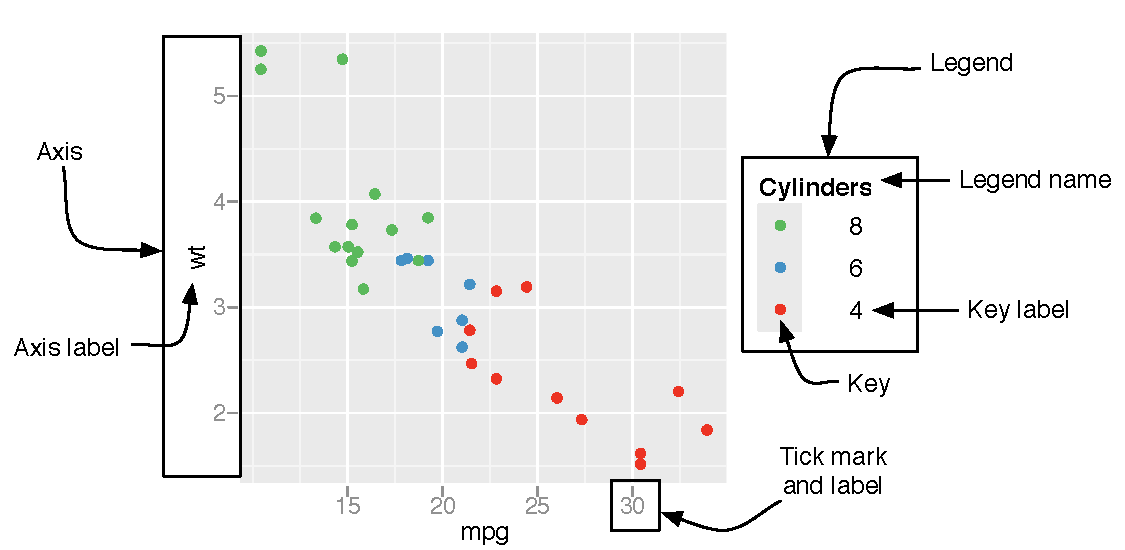
\includegraphics[width=\textwidth]{scale-guides}
  
  \caption{The components of the axes and legend.}
  \label{fig:labelled-guides}
\end{figure}

In \ggplot, legends and axes are produced automatically based on the scales and geoms that you used in the plot. This requires collecting information about how each aesthetic is used. We need the domain of scale for that aesthetic, to determine the value of the legend keys; and a list of the geoms that use that aesthetic, so we know how to draw the keys. For example, the point geom has points in the legend key and the lines geom has lines. If both points and lines are used then both will be drawn.

\ggplot tries to use the smallest possible number of legends that accurately conveys the scales used in the plot.  It does this by combining legends for the same variable with different aesthetics.  Figure~\ref{fig:legend-merge} shows an example of this.  

% In order for legends to be merged, they must have the same title.  For this reason, if you change the title of one of the merged legends you'll need to change it for all of them.

% FIGURE
%  COLS: 3
%  CAPTION: Colour legend, shape legend, colour + shape legend. 
%  LABEL: legend-merge
%
% p <- ggplot(diamonds[1:100, ], aes(x=price, y=carat)) + geom_point() + geom_point() + opts(keep = "legend_box")
% p + aes(colour = cut)
% ggsave(file="_include/lm-1.pdf", width=1.5, height=1.9)
% p + aes(shape = cut)
% ggsave(file="_include/lm-2.pdf", width=1.5, height=1.9)
% p + aes(shape = cut, colour= cut)
% ggsave(file="_include/lm-2.pdf", width=1.5, height=1.9)
% 
\begin{figure}[htbp]
  \centering
  \includegraphics[width=1in]{lm-1}%
  \includegraphics[width=1in]{lm-2}%
  \includegraphics[width=1in]{lm-3}
  
  \caption{Colour legend, shape legend, colour + shape legend. }
  \label{fig:legend-merge}
\end{figure}

\subsection{Customising appearance}

As well as controlling the broader details of the contents of the legends, it is also possible to precisely customise their rendering.  The following arguments and options are particularly useful for that task.

\begin{itemize}
  \item The {\tt breaks} and {\tt labels} arguments to the scale function are particularly important because they control what tick marks appear on the axis and what keys appear on the legend.  If the breaks chosen by default are not appropriate (or you want to use more informative labels) setting these arguments will adjust the appearance of the legend keys and axis tick marks.  
  
  \item The theme settings {\tt axis.box}, {\tt axis.title}, {\tt axis.ticks}, {\tt legend.box}, {\tt legend.title}, and {\tt legend.keys} control the visual appearance of axes and legends.  For more details on how to manipulate these settings, see Section~\ref{sec:theming}.

  \item The internal grid lines are controlled by the breaks and minor breaks arguments.  By default minor grid lines are spaced evenly in the original data space - this gives the common behaviour of log-log plots where major grid lines are multiplicative and minor grid lines are additive.  You can override the minor grid lines with the {\tt minor\_breaks} argument.
  
  \item Position of legends.  Plot level option setting: {\tt legend.position}, can be one of right, left, top or bottom; or none to not display the legend; or a numeric position.  The numeric position gives (in npc  coordinates) the position of the corner given by {\tt legend.justification}.  
  
  \item Position scales also have the {\bf expand} argument, which controls the amount of extra space added to axis limits.  This is a numeric vector of length two: the first number is a multiplicative amount and the second is an additive additive.  The default for continuous scales is {\tt c(0.05, 0)} (i.e.\ add 5\% extra space on each end); for discrete scales it is {\tt c(0, 0.75)}).  Set to {\tt c(0, 0)} to eliminate extra space.
  
\end{itemize}

\section{More resources}
\label{sec:scale_resources}

As you experiment with different aesthetic choices and new scales, it's important to keep in mind how the plot will be perceived.   Some particularly good references to consult are:

\begin{itemize}
  \item \citet{cleveland:1993,cleveland:1987,cleveland:1994} for research on how plots are perceived and the best ways to encode data.
  \item \citet{tufte:2006,tufte:1990,tufte:1997,tufte:2001} for how to make beautiful, data-rich, graphics.
  \item \citet{brewer:1994,brewer:1994a} for how to colours that work well in a wide variety of situations, particularly for area plots.
  \item \citet{carr:1999,carr:1994,carr:2002}, for the use of colour in general.
\end{itemize}

\ifwhole
\else
  \nobibliography{/Users/hadley/documents/phd/references}
  \end{document}
\fi